%%%%%%%%%%%%%%%%%%%%%%%%%%%%%%%%%%%%%%%%%%%%%%%%%%%%%%%%%%%%%%%%%%%%%%%%%%%%%
%
%  System        : 
%  Module        : 
%  Object Name   : $RCSfile$
%  Revision      : $Revision$
%  Date          : $Date$
%  Author        : $Author$
%  Created By    : Robert Heller
%  Created       : Mon Nov 13 11:28:00 2023
%  Last Modified : <231113.1314>
%
%  Description 
%
%  Notes
%
%  History
% 
%%%%%%%%%%%%%%%%%%%%%%%%%%%%%%%%%%%%%%%%%%%%%%%%%%%%%%%%%%%%%%%%%%%%%%%%%%%%%
%
%    Copyright (C) 2023  Robert Heller D/B/A Deepwoods Software
%			51 Locke Hill Road
%			Wendell, MA 01379-9728
%
%    This program is free software; you can redistribute it and/or modify
%    it under the terms of the GNU General Public License as published by
%    the Free Software Foundation; either version 2 of the License, or
%    (at your option) any later version.
%
%    This program is distributed in the hope that it will be useful,
%    but WITHOUT ANY WARRANTY; without even the implied warranty of
%    MERCHANTABILITY or FITNESS FOR A PARTICULAR PURPOSE.  See the
%    GNU General Public License for more details.
%
%    You should have received a copy of the GNU General Public License
%    along with this program; if not, write to the Free Software
%    Foundation, Inc., 675 Mass Ave, Cambridge, MA 02139, USA.
%
% 
%
%%%%%%%%%%%%%%%%%%%%%%%%%%%%%%%%%%%%%%%%%%%%%%%%%%%%%%%%%%%%%%%%%%%%%%%%%%%%%

\documentclass[12pt,twoside]{article}
\usepackage{graphicx}
\usepackage{mathptm}
\usepackage{times}
\usepackage{makeidx}
\usepackage{ifpdf}
\usepackage{footmisc}
\ifpdf
\usepackage[pdftex,
            pagebackref=true,
            colorlinks=true,
            linkcolor=blue,
            unicode
           ]{hyperref}
\else
\usepackage[ps2pdf,
            pagebackref=true,
            colorlinks=true,
            linkcolor=blue,
            unicode
           ]{hyperref}
\usepackage{pspicture}
\fi
\usepackage{url}
\pagestyle{headings}
\makeindex
\emergencystretch=50pt
\setcounter{tocdepth}{3}
\setcounter{secnumdepth}{3}
\title{6 foot (scale) Light Bar Board Instructions}
\author{Robert Heller \\ The Country Robot \\ Wendell, MA, USA}
\date{\today}
\begin{document}
\maketitle


\begin{centering}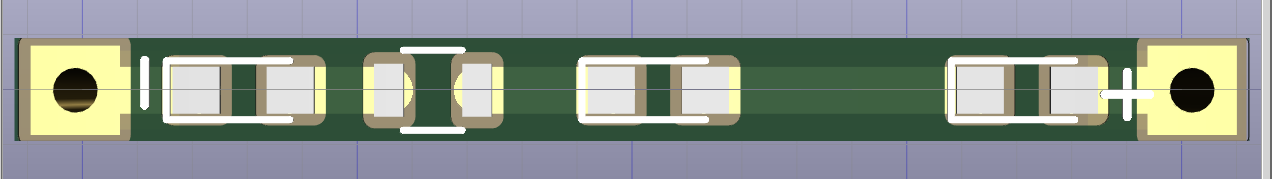
\includegraphics[width=4in]{6footfl3d.png}\\\end{centering}

\begin{centering}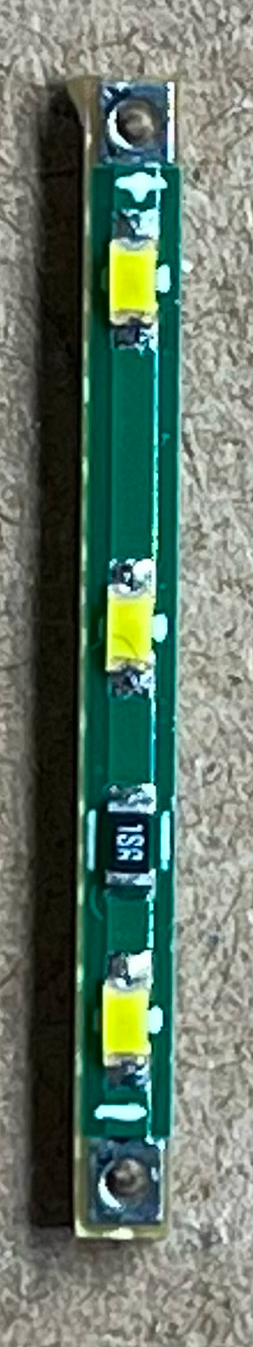
\includegraphics[height=3in]{6footfl_photo.png}\\\end{centering}

This is a LED light bar intended as an overhead light for a pool table, using
a hood. A hood can be 3D printed from the file here: 
\url{https://www.thecountryrobot.com/wp-content/uploads/2023/11/hood.zip}\\
\includegraphics[height=1in]{hood\_qr\_download.png}.

The light bar can also be used anywhere a linear 6 foot florescent or LED light
fixture might be used. The light bar has 3 white SMD LEDs with a series
resistor and is intended for a 12V supply. Can be driven from a MCU with a
driver using PWM to adjust brightness. 

\section{Connecting the board}

The board has two (2) through hole solder pads. They are labeled with plus (+) 
and minus (-) signs.  Typically wires can be fed from the back side of the 
board and soldered on the front side.  These wires can be used to suspend the 
board from a ceiling.

\end{document}
